\begin{frame}
\frametitle{Objectives}

Tools that help in analysing any one-dimensional discrete structures in a generic framework. 

  \begin{block}{Examples in digital geometry}
    \begin{itemize}
    \item digital curves
      \begin{itemize}
      \item 2d, 3d, nd
      \item 4-connected, 8-connected, disconnected
      \item pixels, interpixels, points
      \item open or closed
      \end{itemize}
		\item chain codes
    \end{itemize}
  \end{block}

\alert{Constant structures, not mutable} 

\end{frame}

\section{Iterators/Circulators and Ranges}


\begin{frame}
  \frametitle{Structures}

  \begin{block}{2 characteristics}
    \begin{itemize}
		\item discrete
    \item one-dimensional
    \end{itemize}
  \end{block}

  \begin{block}{2 notions}
    \begin{itemize}
    \item element
    \item local order (next and previous element)
    \end{itemize}
  \end{block}



\end{frame}

\begin{frame}
  \frametitle{Iterators}

  \begin{block}{Iterator}
    \begin{itemize}
    \item operator* (to get the element)
    \item operator++, operator- - (to point to the next and previous element)
    \end{itemize}
  \end{block}

  \begin{block}{Reachability}
An iterator j is reachable from an iterator i if and only if i can be made equal to j with finitely many applications of the operator++. 
  \end{block}

  \begin{block}{Range}
If j is reachable from i, one can iterate over the range of elements bounded by i and j, from the one pointed to by i and up to but not including the one pointed to by j. Such a range is valid and is denoted by [i,j).
  \end{block}

\end{frame}

\begin{frame}
  \frametitle{Open/Linear structures}

  \begin{block}{Classic iterator}
\begin{itemize}
  \item past-the-end value
  \item $[begin,end)$ is the whole range
  \item $[i,j)$ is not always valid
  \item $[i,i)$ is the empty range
\end{itemize}
  \end{block}

%image
 \begin{center}
   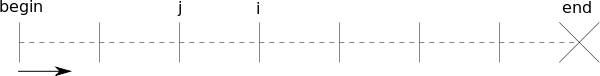
\includegraphics[width=1\textwidth]{linearRange}
 \end{center}

\end{frame}

\begin{frame}
  \frametitle{Closed/Circular structures}

  \begin{block}{CGAL circular iterator (circulator)}
\begin{itemize}
  \item no past-the-end value
  \item $[i,j)$ is always valid
  \item $[i,i)$ is the whole range
  \item As long as $i \neq j$, the range $[i,j)$ behaves like a classic iterator range. 
\end{itemize}
  \end{block}

%image
 \begin{center}
   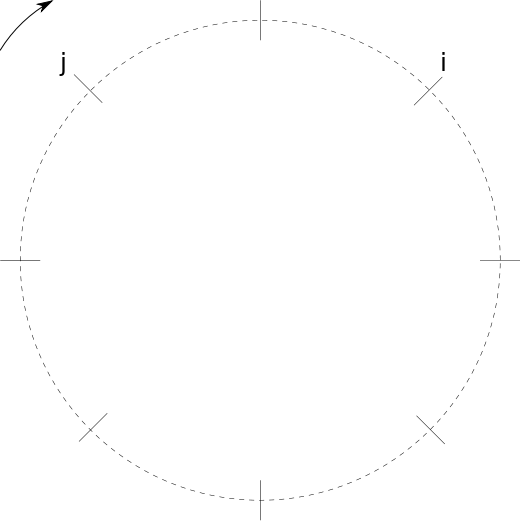
\includegraphics[width=0.6\textwidth]{circularRange}
 \end{center}

\end{frame}

\begin{frame}
  \frametitle{Scanning backward}

  \begin{block}{Reverse iterator}
A reverse iterator is an adaptor for scanning backward. The operator++ of the adaptor calls the operator-- of the underlying (circular)iterator and conversely. You can use the STL reverse iterator.
  \end{block}

  \begin{block}{Tricky part}
Operator* of the adaptor calls operator- - of the underlying (circular)iterator before calling its operator*.
  \end{block}

%image
 \begin{center}
   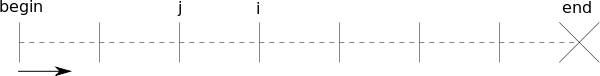
\includegraphics[width=1\textwidth]{linearRange}
 \end{center}

\end{frame}


\section{Classes}

\begin{frame}
  \frametitle{GridCurve}

  \begin{block}{}
GridCurve is an (open or closed) n-dimensional oriented grid curve. It stores a list of alternated (signed) 0-cells and 1-cells. 
  \end{block}

%image
 \begin{center}
   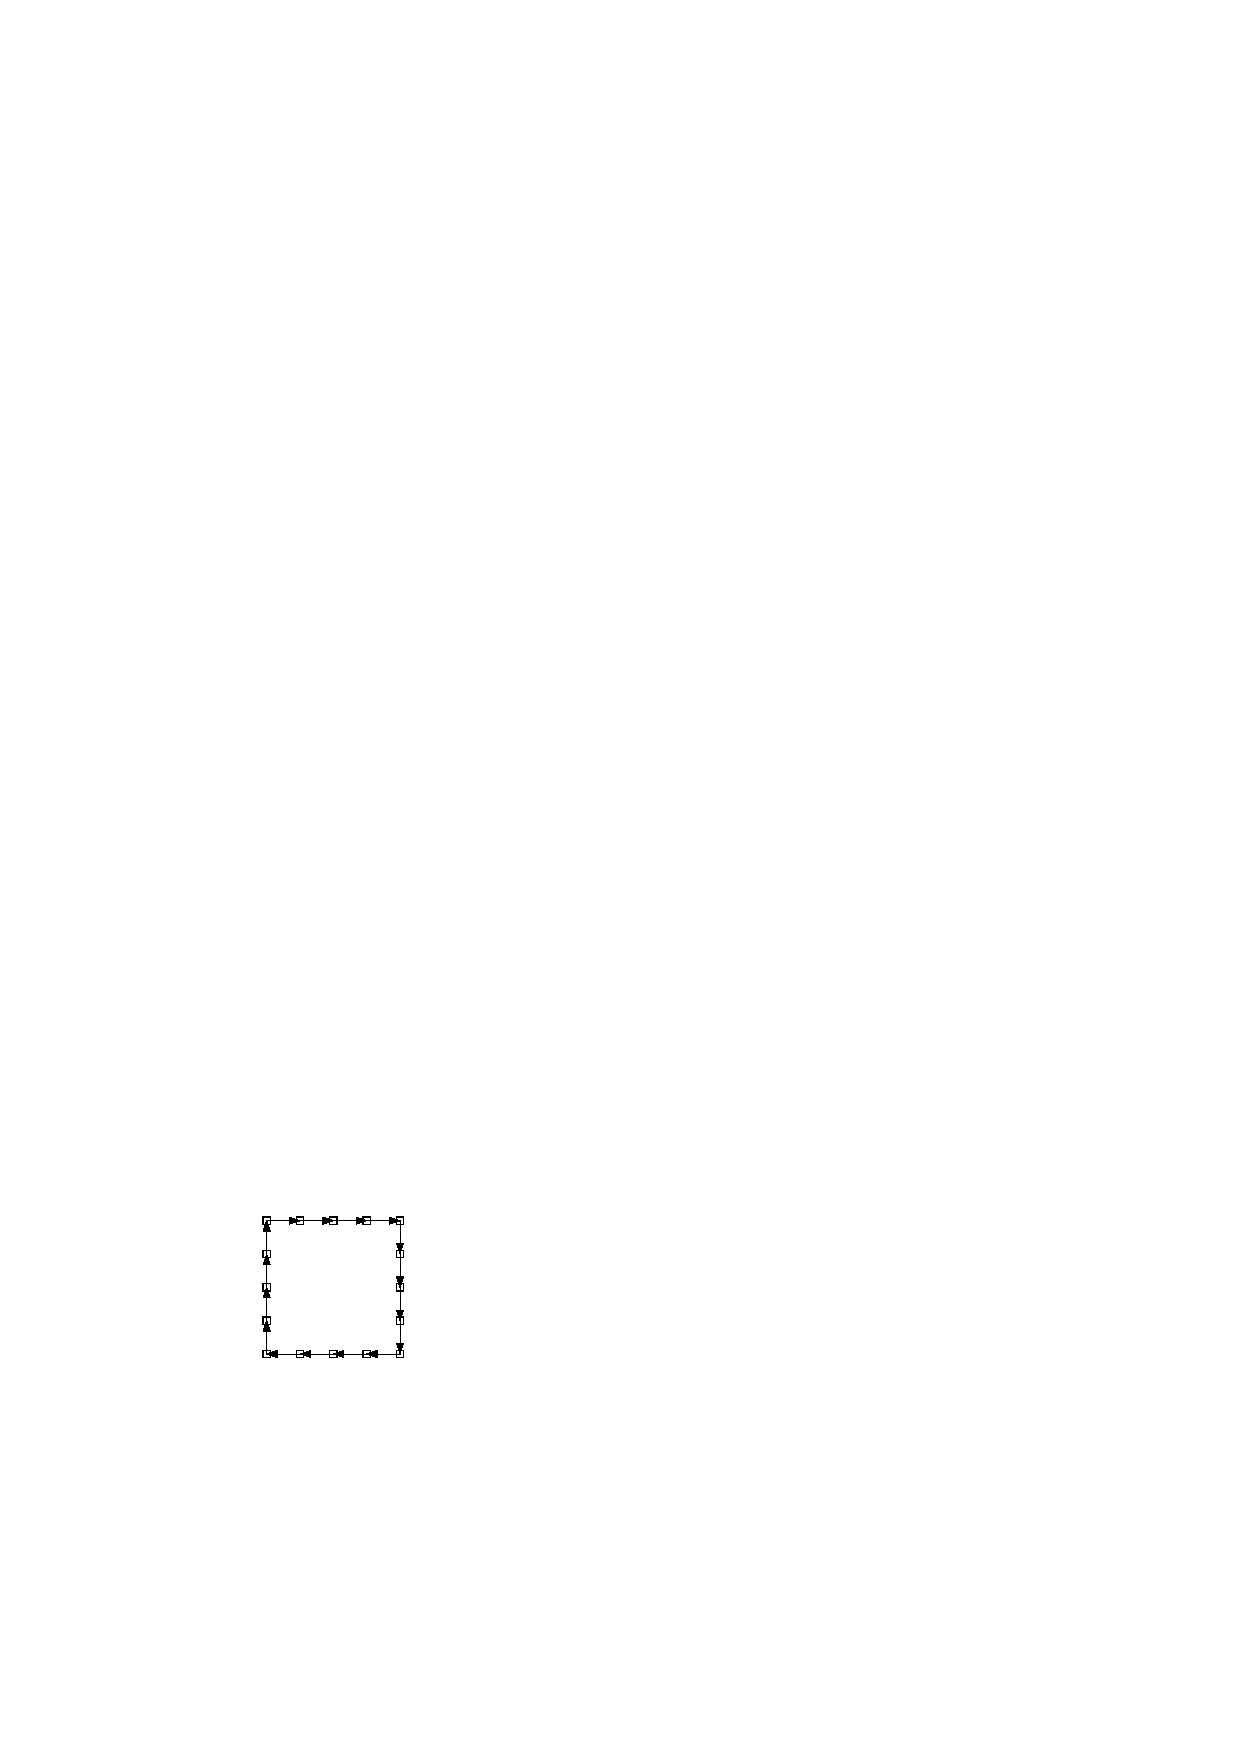
\includegraphics[width=0.5\textwidth,page=1]{gridcurve}
 \end{center}

\end{frame}

\begin{frame}
  \frametitle{GridCurve}

  \begin{block}{Ranges}
GridCurve provides many ranges as nested types to iterate over different kinds of elements:
\begin{itemize}
 \item nd
  \begin{itemize}
   \item<1-2> SCellsRange
   \item<3> PointsRange
   \item<4> MidPointsRange
   \item<5> ArrowsRange
  \end{itemize}
 \item 2d TODO
  \begin{itemize}
   \item<6> InnerPointsRange
   \item<7> OuterPointsRange
   \item<8> IncidentPointsRange
   \item CodesRange
  \end{itemize}
\end{itemize}
  \end{block}

\only<1>{
 \begin{center}
   \includegraphics[width=0.25\textwidth,page=2]{gridcurve}
 \end{center}
}
\only<2>{
 \begin{center}
   \includegraphics[width=0.25\textwidth,page=3]{gridcurve}
 \end{center}
}
\only<3>{
 \begin{center}
   \includegraphics[width=0.25\textwidth,page=5]{gridcurve}
 \end{center}
}
\only<4>{
 \begin{center}
   \includegraphics[width=0.25\textwidth,page=4]{gridcurve}
 \end{center}
}
\only<5>{
 \begin{center}
   \includegraphics[width=0.25\textwidth,page=6]{gridcurve}
 \end{center}
}
\only<6>{
 \begin{center}
   \includegraphics[width=0.25\textwidth,page=7]{gridcurve}
 \end{center}
}
\only<7>{
 \begin{center}
   \includegraphics[width=0.25\textwidth,page=8]{gridcurve}
 \end{center}
}
\only<8>{
 \begin{center}
   \includegraphics[width=0.25\textwidth,page=9]{gridcurve}
 \end{center}
}
\end{frame}

\begin{frame}
  \frametitle{Code}

  \begin{block}{FreemanChain}
FreemanChain is 2-dimensional and 4-connected digital curve stored as a string of codes {0,1,2,3}. 
As GridCurve, it provides a CodesRange.
  \end{block}

  \begin{block}{Conversion between FreemanChain and GridCurve}
TODO
  \end{block}

\end{frame}


